% !TEX TS-program = xelatex
% !TEX encoding = UTF-8
% !Mode:: "TeX:UTF-8"

\documentclass[onecolumn, oneside, ctexart]{SUSTechHomework}
\setlength{\parindent}{2em}
\linespread{1.5}
\usepackage{karnaugh-map}
\usepackage{float}
\usepackage{multicol}
\usepackage{longtable}
\usepackage{circuitikz}
\ctikzset{logic ports=ieee}
\usetikzlibrary{calc}

\coursecode{CS207}
\coursename{Digital Logic}
\title{Assignment 3}
\date{Dec. 6, 2021}

\lstset{language=verilog}

\begin{document}
  \maketitle
\section{DIGITAL DESIGN THEORY}

\subsection*{Q. 1}
\vspace{-2em}
\begin{center}
\begin{karnaugh-map}[4][4][1][$CD$][$AB$]
\minterms{0, 1, 5, 8, 9, 10, 11, 13, 15}
\implicant{1}{9}
\implicant{13}{11}
\implicant{8}{10}
\implicantedge{0}{1}{8}{9}
\end{karnaugh-map}
\begin{karnaugh-map}[4][4][1][$CD$][$AB$]
\maxterms{2,3,4,6,7,12,14}
\implicant{3}{6}
\implicantedge{4}{12}{6}{14}
\end{karnaugh-map}
\end{center}
\vspace{-2.5em}
\paragraph{(a)}$F(A,B,C,D)=B'C'+C'D+AD+AB'$
\vspace{-1em}
\paragraph{(b)}$F(A,B,C,D)=(B+C)'+(C+D')'+(A'+D')'+(A'+B)'$
\vspace{-1em}
\paragraph{(c)}$F(A,B,C,D)=((B'C')'(C'D)'(AD)'(AB')')'$
\vspace{-1em}
\paragraph{(d)}$F(A,B,C,D)=(B'+D)(A+C')$
\vspace{-1em}
\paragraph{(e)}$F(A,B,C,D)=((B'+D)'+(A+C')')'$
\vspace{-1em}
\paragraph{(f)}$F(A,B,C,D)=(BD')'(A'C)'$
\subsection*{Q. 2}
\subsubsection*{Four-bit Parity Generator}
\vspace{-1.2em}
\begin{longtable}[c]{cccc|c}
\multicolumn{4}{l|}{Input 4-bit message} & \multicolumn{1}{l}{Odd parity generator} \\ \hline
\endfirsthead
%
\endhead
%
\hline
\endfoot
%
\endlastfoot
%
A        & B        & C        & D       & P                                        \\ \hline
0        & 0        & 0        & 0       & 1                                        \\
0        & 0        & 0        & 1       & 0                                        \\
0        & 0        & 1        & 0       & 0                                        \\
0        & 0        & 1        & 1       & 1                                        \\
0        & 1        & 0        & 0       & 0                                        \\
0        & 1        & 0        & 1       & 1                                        \\
0        & 1        & 1        & 0       & 1                                        \\
0        & 1        & 1        & 1       & 0                                        \\
1        & 0        & 0        & 0       & 0                                        \\
1        & 0        & 0        & 1       & 1                                        \\
1        & 0        & 1        & 0       & 1                                        \\
1        & 0        & 1        & 1       & 0                                        \\
1        & 1        & 0        & 0       & 1                                        \\
1        & 1        & 0        & 1       & 0                                        \\
1        & 1        & 1        & 0       & 0                                        \\
1        & 1        & 1        & 1       & 1                                        \\ \hline
\end{longtable}
\begin{center}
\begin{karnaugh-map}[4][4][1][$CD$][$AB$]
\minterms{0,3,5,6,9,10,12,15}
\implicant{0}{0}
\implicant{3}{3}
\implicant{5}{5}
\implicant{6}{6}
\implicant{9}{9}
\implicant{10}{10}
\implicant{12}{12}
\implicant{15}{15}
\end{karnaugh-map}
\end{center}
\vspace{-2.5em}
\begin{align*}
F(A,B,C,D)&=A'B'C'D'+A'B'CD+A'BC'D+A'BCD'+ABC'D'+ABCD+AB'C'D+AB'CD'\\
&=A'D'(BC+B'C')+A'D(B'C+BC')+AD'(BC'+B'C)+AD(BC+B'C')\\
&=A'D'(B\oplus C)'+A'D(B\oplus C)+AD'(B\oplus C)+AD(B\oplus C)'\\
&=(A'D'+AD)(B\oplus C)'+(A'D+AD')(B\oplus C)\\
&=(A\oplus D)'(B\oplus C)'+(A\oplus D)(B\oplus C)\\
&=((A\oplus D)\oplus (B\oplus C))'
\end{align*}
\centerline{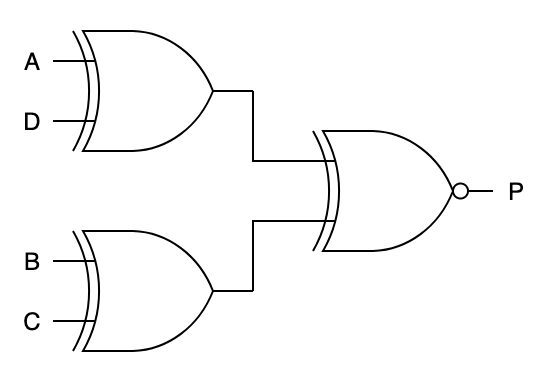
\includegraphics[width=0.4\textwidth]{fig/f21}}


\subsubsection*{Three-bit Parity Checker}
\vspace{-1.2em}
% Please add the following required packages to your document preamble:
% \usepackage{longtable}
% Note: It may be necessary to compile the document several times to get a multi-page table to line up properly
\begin{longtable}[c]{cccc|c}
\multicolumn{4}{l|}{Input (3+1)-bit} & \multicolumn{1}{l}{Odd parity checker} \\ \hline
\endfirsthead
%
\endhead
%
\hline
\endfoot
%
\endlastfoot
%
A       & B       & C       & P      & $C_P$                                   \\ \hline
0       & 0       & 0       & 0      & 1                                      \\
0       & 0       & 0       & 1      & 0                                      \\
0       & 0       & 1       & 0      & 0                                      \\
0       & 0       & 1       & 1      & 1                                      \\
0       & 1       & 0       & 0      & 0                                      \\
0       & 1       & 0       & 1      & 1                                      \\
0       & 1       & 1       & 0      & 1                                      \\
0       & 1       & 1       & 1      & 0                                      \\
1       & 0       & 0       & 0      & 0                                      \\
1       & 0       & 0       & 1      & 1                                      \\
1       & 0       & 1       & 0      & 1                                      \\
1       & 0       & 1       & 1      & 0                                      \\
1       & 1       & 0       & 0      & 1                                      \\
1       & 1       & 0       & 1      & 0                                      \\
1       & 1       & 1       & 0      & 0                                      \\
1       & 1       & 1       & 1      & 1                                      \\ \hline
\end{longtable}
\begin{center}
\begin{karnaugh-map}[4][4][1][$CP$][$AB$]
\minterms{0,3,5,6,9,10,12,15}
\implicant{0}{0}
\implicant{3}{3}
\implicant{5}{5}
\implicant{6}{6}
\implicant{9}{9}
\implicant{10}{10}
\implicant{12}{12}
\implicant{15}{15}
\end{karnaugh-map}
\end{center}
\vspace{-2.5em}
\begin{align*}
F(A,B,C,P)&=A'B'C'P'+A'B'CP+A'BC'P+A'BCP'+ABC'P'+ABCP+AB'C'P+AB'CP'\\
&=A'P'(BC+B'C')+A'P(B'C+BC')+AP'(BC'+B'C)+AP(BC+B'C')\\
&=A'P'(B\oplus C)'+A'P(B\oplus C)+AP'(B\oplus C)+AP(B\oplus C)'\\
&=(A'P'+AP)(B\oplus C)'+(A'P+AP')(B\oplus C)\\
&=(A\oplus P)'(B\oplus C)'+(A\oplus P)(B\oplus C)\\
&=((A\oplus P)\oplus (B\oplus C))'
\end{align*}
\centerline{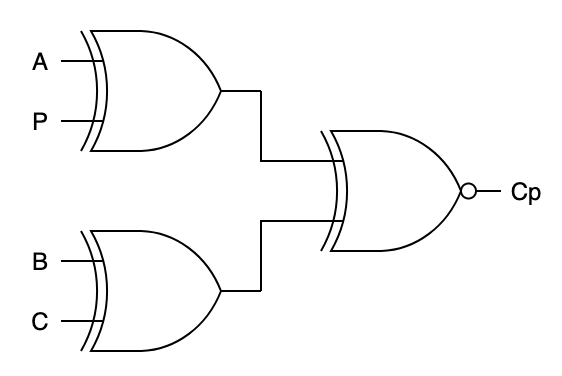
\includegraphics[width=0.4\textwidth]{fig/f22}}

\subsection*{Q. 3}
\begin{longtable}[c]{ccc|ccc}
\multicolumn{3}{c}{Input\quad} & \multicolumn{3}{|c}{Output\quad} \\ \hline
\endfirsthead
%
\endhead
%
\hline
\endfoot
%
\endlastfoot
%
x       & y       & z      & A       & B       & C      \\ \hline
0       & 0       & 0      & 0       & 1       & 0      \\
0       & 0       & 1      & 0       & 1       & 1      \\
0       & 1       & 0      & 1       & 0       & 0      \\
0       & 1       & 1      & 1       & 0       & 1      \\
1       & 0       & 0      & 0       & 1       & 1      \\
1       & 0       & 1      & 1       & 0       & 0      \\
1       & 1       & 0      & 1       & 0       & 1      \\
1       & 1       & 1      & 1       & 1       & 0      \\ \hline
\end{longtable}

\begin{center}
\begin{karnaugh-map}[4][2][1][$xy$][$z$]
\minterms{1,5,6,3,7}
\implicant{1}{7}
\implicant{7}{6}
\end{karnaugh-map}

\begin{karnaugh-map}[4][2][1][$xy$][$z$]
\minterms{0,4,2,7}
\implicant{0}{4}
\implicantedge{0}{0}{2}{2}
\implicant{7}{7}
\end{karnaugh-map}

\begin{karnaugh-map}[4][2][1][$xy$][$z$]
\minterms{4,3,2,5}
\implicant{4}{5}
\implicant{3}{2}
\end{karnaugh-map}
\end{center}
\vspace{-2em}
\begin{align*}
A&=y+xz\\
B&=x'y'+y'z'+xyz\\
&=(x'+z')y'+(xz)y\\
&=(xz)'y'+(xz)y\\
&=((xz)\oplus y)'\\
C&=xz'+x'z\\
&=x\oplus z
\end{align*}
\centerline{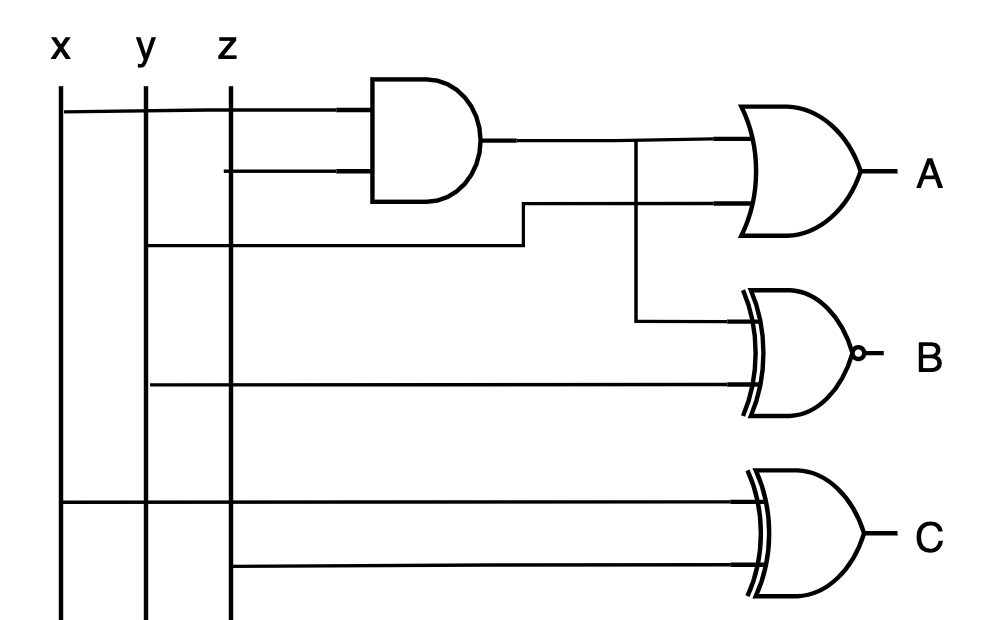
\includegraphics[width=0.4\textwidth]{fig/q3}}

\subsection*{Q. 4}
\begin{longtable}[c]{llllll}
         &          &          & $A_2$    & $A_1$    & $A_0$    \\
\endfirsthead
%
\endhead
%
$\times$ &          &          & $B_2$    & $B_1$    & $B_0$    \\ \hline
         &          &          & $A_2B_0$ & $A_1B_0$ & $A_0B_0$ \\
         &          & $A_2B_1$ & $A_1B_1$ & $A_0B_1$ &          \\
         & $A_2B_2$ & $A_1B_2$ & $A_0B_2$ &          &          \\ \hline
$C_5$\quad & $C_4$    & $C_3$    & $C_2$    & $C_1$    & $C_0$   
\end{longtable}
\par Starting with the traditional vertical multiplication, we found out that: \ding{172} a 3-bit multiplication is made up of three partial products; \ding{173} each partial product, is a 1-bit $\times$ 3-bit, while bits can only be 0 or 1, this multiplication doesn't have carry out, and thus can simply use three; \emph{and gate} to denote them \ding{174} the partial products are added up to give the final result. Formally, we say:
\begin{align*}
C_0&=A_0B_0&\text{(no carry out)}\\
\{\text{Carry}_1, C_1\}&=A_1B_0+A_0B_1&\text{LHS = 2 $\times$ Carry$_1$ + $C_1$}\\
\{\text{Carry}_2, C_2\}&=A_2B_0+A_1B_1+A_0B_2+\text{Carry}_1\\
\cdots\\
\{\text{Carry}_4, C_4\}&=A_2B_2+\text{Carry}_3\\
C_5&=\text{Carry}_4
\end{align*}
\par A.k.a., since multiply takes \emph{AND} operation of the all binary combination from the bits of A and B and add the result with shifting \emph{i+j (i,j denotes the indices of bits in A and B)} operations. To express the final result in binary form, we only take the least bit of output sum and feed the rest bits of output sum together with the carry out bit into the augend input of the next full adder. \\
\vspace{1em}
\centerline{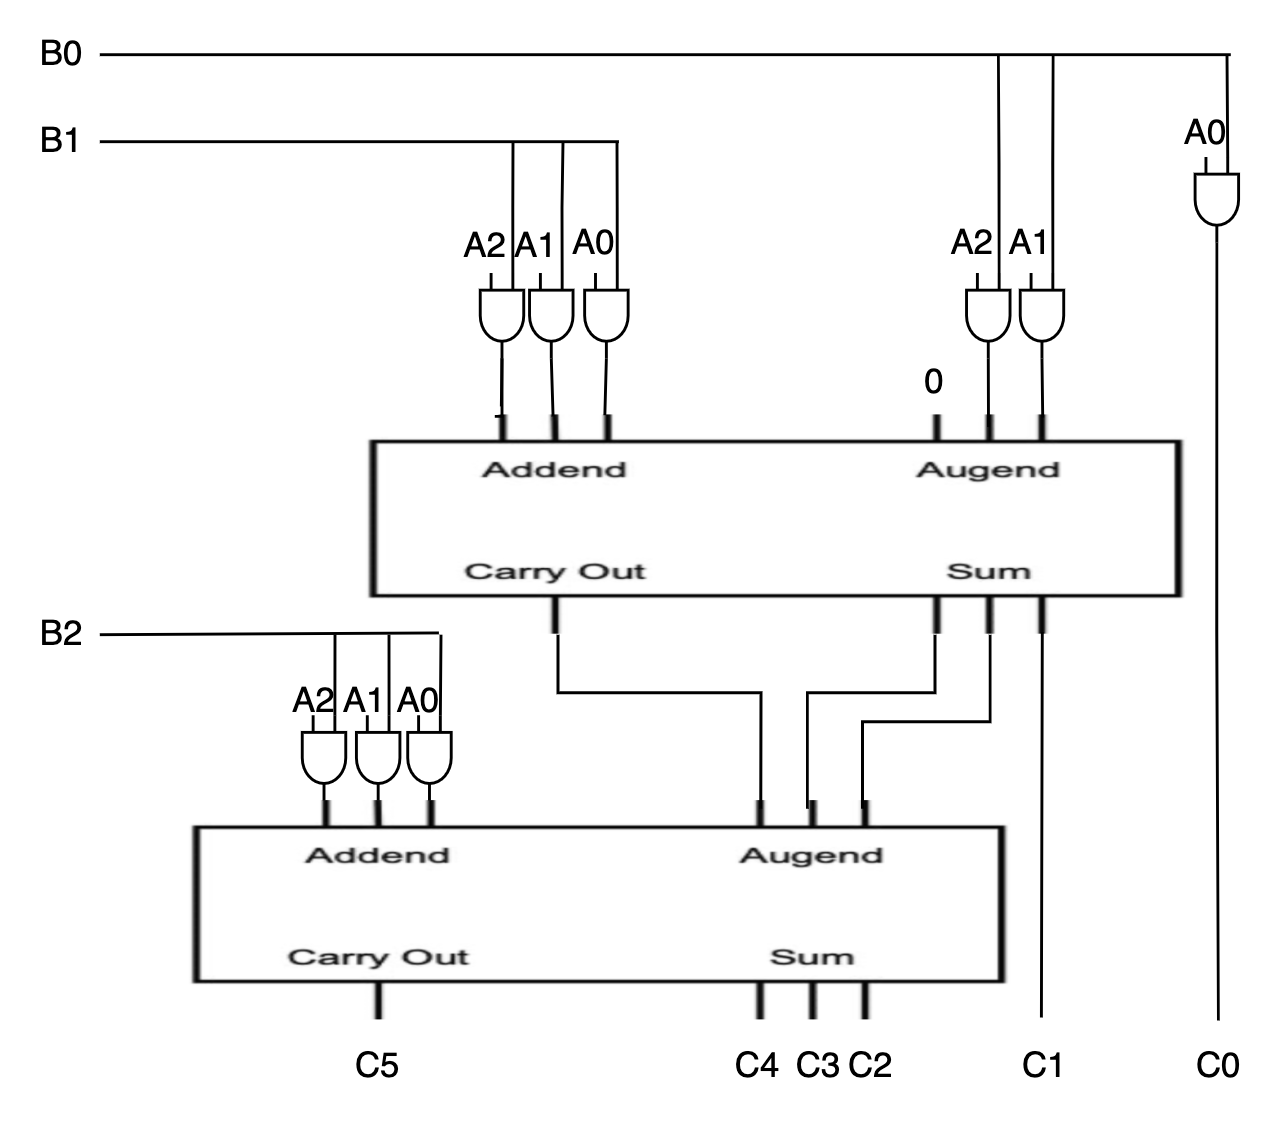
\includegraphics[width=0.5\textwidth]{fig/q4}}

\par The circuit can be represented as the following logic formulas:
\begin{align*}
C_0&=A_0B_0\\
C_1&=(A_1B_0)\oplus(A_0B_1)\\
C_2&=(A_2B_0)\oplus(A_1B_1)\oplus(A_0B_2)\oplus(A_1B_0A_0B_1)\\
C_3&=(A_2B_1)\oplus(A_1B_2)\oplus(A_2B_0A_1B_1A_0B_2B_0)\\
C_4&=(A_2B_2)\oplus(A_2B_0A_1B_1A_0B_2B_0)\\
C_5&=A_2B_0A_1B_1A_0B_2B_0
\end{align*}
\vspace{-2em}

\subsection*{Q. 5}
\paragraph{(a)}$F(A, B, C, D)=\Sigma(1, 3, 5, 8, 10, 14)$
\par D1, D3, D5, D8, D10, D14 should be connected to \emph{signal 1}, while the left ports (D0, D2, D4, D6, D7, D9, D11, D12, D13, D15) should be connected to \emph{signal 0}.
\paragraph{(b)}$F(A, B, C, D)=\Pi(4, 7, 11)=\Sigma(0, 1, 2, 3, 5, 6, 8, 9, 10, 12, 13, 14, 15)$
\par D4, D7, D11 should be connected to \emph{signal 0}, while the left ports (D0, D1, D2, D3, D5, D6, D8, D9, D10, D12, D13, D14, D15) should be connected to \emph{signal 1}.
\subsection*{Q. 6}
\begin{longtable}[c]{ccc|cc}
\multicolumn{3}{c|}{Input\quad} & \multicolumn{2}{c}{Output\quad} \\ \hline
\endfirsthead
%
\endhead
%
\hline
\endfoot
%
\endlastfoot
%
X     & Y    & $B_{in}$    & Diff      & $B_{out}$      \\ \hline
0     & 0    & 0           & 0         & 0              \\
0     & 0    & 1           & 1         & 1              \\
0     & 1    & 0           & 1         & 1              \\
0     & 1    & 1           & 0         & 1              \\
1     & 0    & 0           & 1         & 0              \\
1     & 0    & 1           & 0         & 0              \\
1     & 1    & 0           & 0         & 0              \\
1     & 1    & 1           & 1         & 1              \\ \hline
\end{longtable}
\centerline{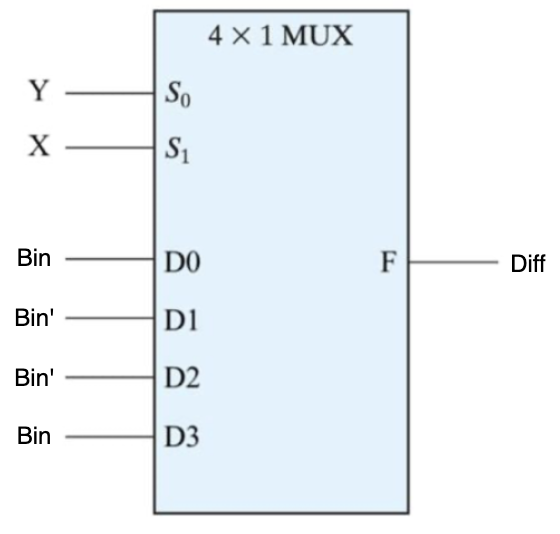
\includegraphics[width=0.3\textwidth]{fig/q61}\qquad 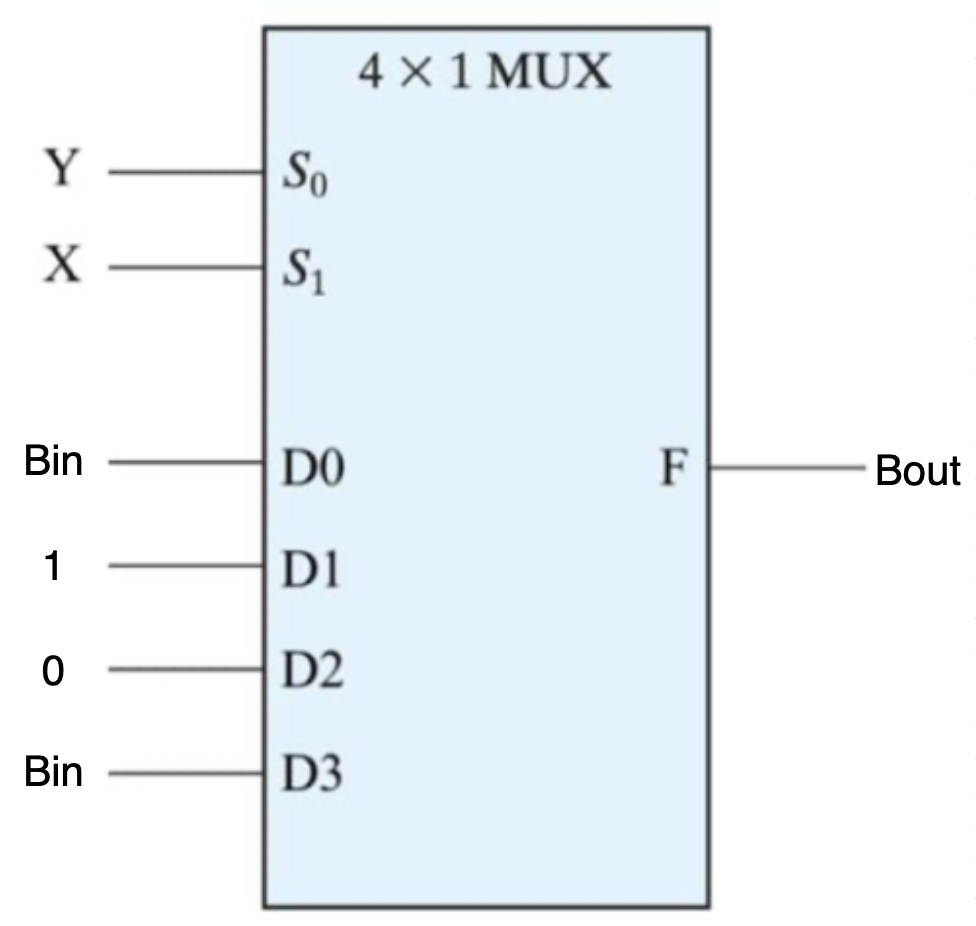
\includegraphics[width=0.3\textwidth]{fig/q62}}


\section{DIGITAL DESIGN LAB}

\subsection*{Task 1}
\subsubsection*{Design File}
\begin{lstlisting}
`timescale 1ns/1ps

module decode_74138(
    input A, B, C,
    input G1, G2a, G2b,
    output reg [7:0] Y
);
    always @ * begin
        if ({G1, G2a, G2b} == 'b100) begin
            case ({C, B, A})
                'd0: Y <= ~'b0000_0001;
                'd1: Y <= ~'b0000_0010;
                'd2: Y <= ~'b0000_0100;
                'd3: Y <= ~'b0000_1000;
                'd4: Y <= ~'b0001_0000;
                'd5: Y <= ~'b0010_0000;
                'd6: Y <= ~'b0100_0000;
                'd7: Y <= ~'b1000_0000;
            endcase
        end
        else begin
            Y = ~'b0000_0000;
        end
    end
endmodule


module decode_4_16(
    input A, B, C, D,
    input dec_en,
    output [15:0] Y
);
    reg [2:0] lo_en = 'b000;
    reg [2:0] hi_en = 'b000;
    decode_74138 lo(A, B, C, lo_en[2], lo_en[1], lo_en[0], Y[7:0]);
    decode_74138 hi(A, B, C, hi_en[2], hi_en[1], hi_en[0], Y[15:8]);

        always @ * begin
        if (dec_en) begin
            if (!D) begin
                lo_en <= 'b100;
                hi_en <= 'b000;
            end
            else begin
                lo_en <= 'b000;
                hi_en <= 'b100;
            end
        end
        else begin
            lo_en <= 'b000;
            hi_en <= 'b000;
        end
    end
endmodule
\end{lstlisting}
\vspace{-2em}
\subsubsection*{Simulation File}
\begin{lstlisting}
`timescale 1ns/1ps

module decode_74138_test();
    reg A, B, C;
    reg G1, G2a, G2b;
    wire [7:0] Y;

    decode_74138 dec(A, B, C, G1, G2a, G2b, Y);

    initial begin
        {G1, G2a, G2b} = 'b000;

        while ({G1, G2a, G2b} < 'b111) begin
            {C, B, A} = 'b000;

            while ({C, B, A} < 'b111) begin
                #10 {C, B, A} = {C, B, A} + 1;
            end
            #10 {G1, G2a, G2b} = {G1, G2a, G2b} + 1;
        end
        #10 $finish();
    end
endmodule
\end{lstlisting}
\vspace{-2em}
\centerline{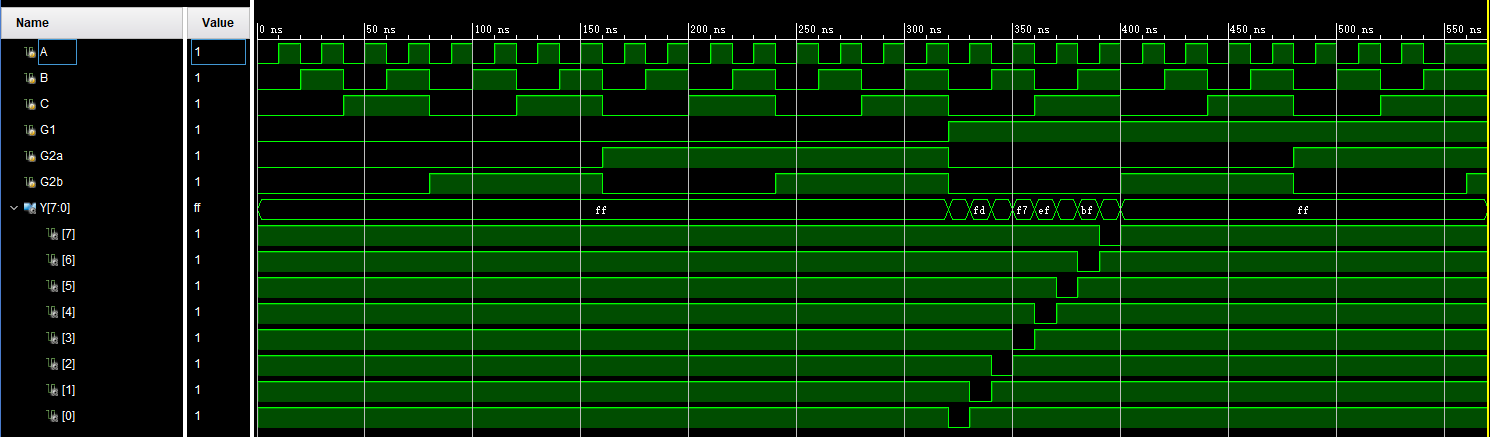
\includegraphics[width=\textwidth]{fig/t1}}
\par The 74138 decoder has three enable ports and should only be enabled when \textbf{\{G1, G2a, G2b\} = 'b100}, when the decoder is not enabled, no matter what the input is, the output keeps 'b1111\_1111. Notice the part of waveform where \textbf{\{G1, G2a, G2b\} = 'b100}, we have \{C, B, A\} be the selection signals and the outputs are all as expected.\\

\begin{lstlisting}
`timescale 1ns/1ps

module decode_4_16_test();
    reg A, B, C, D;
    reg dec_en;
    wire [15:0] Y;

    decode_4_16 dec(A, B, C, D, dec_en, Y);

    initial begin
        dec_en = 'b0;
        repeat(2) begin
            {D, C, B, A} = 'b0000;

            while ({D, C, B, A} < 'b1111) begin
                #10 {D, C, B, A} = {D, C, B, A} + 1;
            end

            #10 dec_en = dec_en + 1;
        end
        #10 $finish();
    end
endmodule
\end{lstlisting}
\vspace{-2em}
\centerline{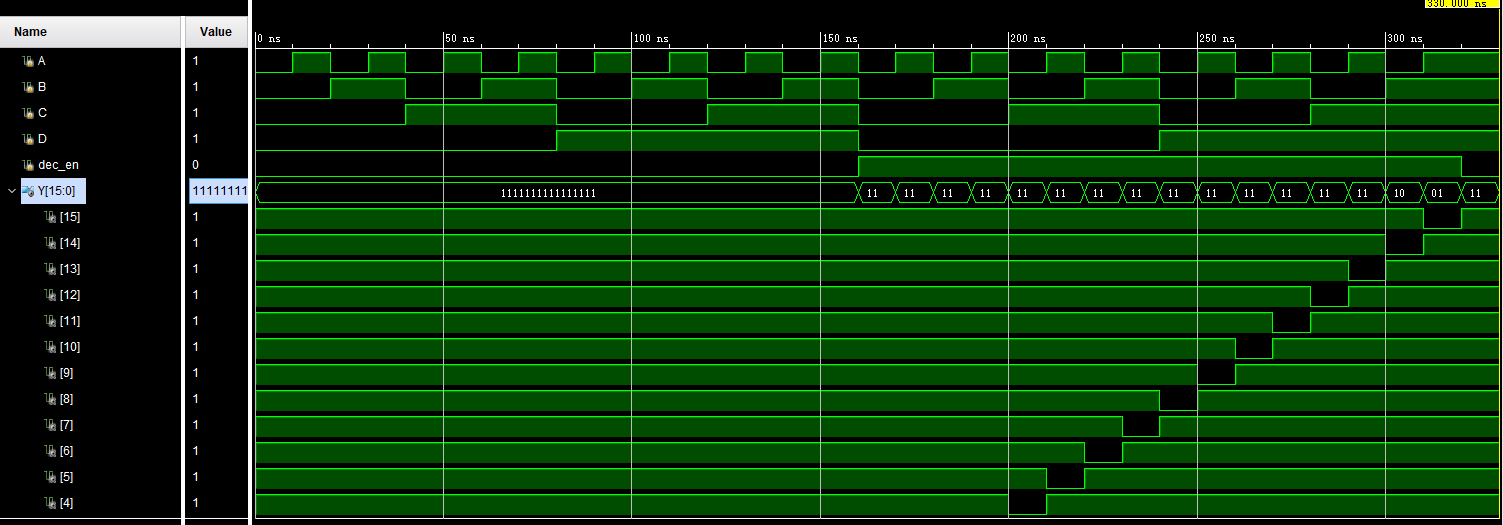
\includegraphics[width=\textwidth]{fig/t2}}
\par Similarly, when the decoder is not enabled, the output keeps 1111\_1111\_1111\_1111, otherwise it fits the result we expected (one-hot).

\subsubsection*{Constraint File}
\begin{lstlisting}
set_property IOSTANDARD LVCMOS33 [get_ports {Y[0]}]
set_property IOSTANDARD LVCMOS33 [get_ports {Y[1]}]
set_property IOSTANDARD LVCMOS33 [get_ports {Y[2]}]
set_property IOSTANDARD LVCMOS33 [get_ports {Y[3]}]
set_property IOSTANDARD LVCMOS33 [get_ports {Y[4]}]
set_property IOSTANDARD LVCMOS33 [get_ports {Y[5]}]
set_property IOSTANDARD LVCMOS33 [get_ports {Y[6]}]
set_property IOSTANDARD LVCMOS33 [get_ports {Y[7]}]
set_property IOSTANDARD LVCMOS33 [get_ports {Y[8]}]
set_property IOSTANDARD LVCMOS33 [get_ports {Y[9]}]
set_property IOSTANDARD LVCMOS33 [get_ports {Y[10]}]
set_property IOSTANDARD LVCMOS33 [get_ports {Y[11]}]
set_property IOSTANDARD LVCMOS33 [get_ports {Y[12]}]
set_property IOSTANDARD LVCMOS33 [get_ports {Y[13]}]
set_property IOSTANDARD LVCMOS33 [get_ports {Y[14]}]
set_property IOSTANDARD LVCMOS33 [get_ports {Y[15]}]
set_property IOSTANDARD LVCMOS33 [get_ports A]
set_property IOSTANDARD LVCMOS33 [get_ports B]
set_property IOSTANDARD LVCMOS33 [get_ports C]
set_property IOSTANDARD LVCMOS33 [get_ports D]
set_property IOSTANDARD LVCMOS33 [get_ports dec_en]
set_property PACKAGE_PIN U5 [get_ports dec_en]
set_property PACKAGE_PIN T5 [get_ports D]
set_property PACKAGE_PIN T4 [get_ports C]
set_property PACKAGE_PIN R4 [get_ports B]
set_property PACKAGE_PIN W4 [get_ports A]
set_property PACKAGE_PIN A21 [get_ports {Y[0]}]
set_property PACKAGE_PIN E22 [get_ports {Y[1]}]
set_property PACKAGE_PIN D22 [get_ports {Y[2]}]
set_property PACKAGE_PIN E21 [get_ports {Y[3]}]
set_property PACKAGE_PIN D21 [get_ports {Y[4]}]
set_property PACKAGE_PIN G21 [get_ports {Y[5]}]
set_property PACKAGE_PIN G22 [get_ports {Y[6]}]
set_property PACKAGE_PIN F21 [get_ports {Y[7]}]
set_property PACKAGE_PIN J17 [get_ports {Y[8]}]
set_property PACKAGE_PIN L14 [get_ports {Y[9]}]
set_property PACKAGE_PIN L15 [get_ports {Y[10]}]
set_property PACKAGE_PIN L16 [get_ports {Y[11]}]
set_property PACKAGE_PIN K16 [get_ports {Y[12]}]
set_property PACKAGE_PIN M15 [get_ports {Y[13]}]
set_property PACKAGE_PIN M16 [get_ports {Y[14]}]
set_property PACKAGE_PIN M17 [get_ports {Y[15]}]
\end{lstlisting}

\centerline{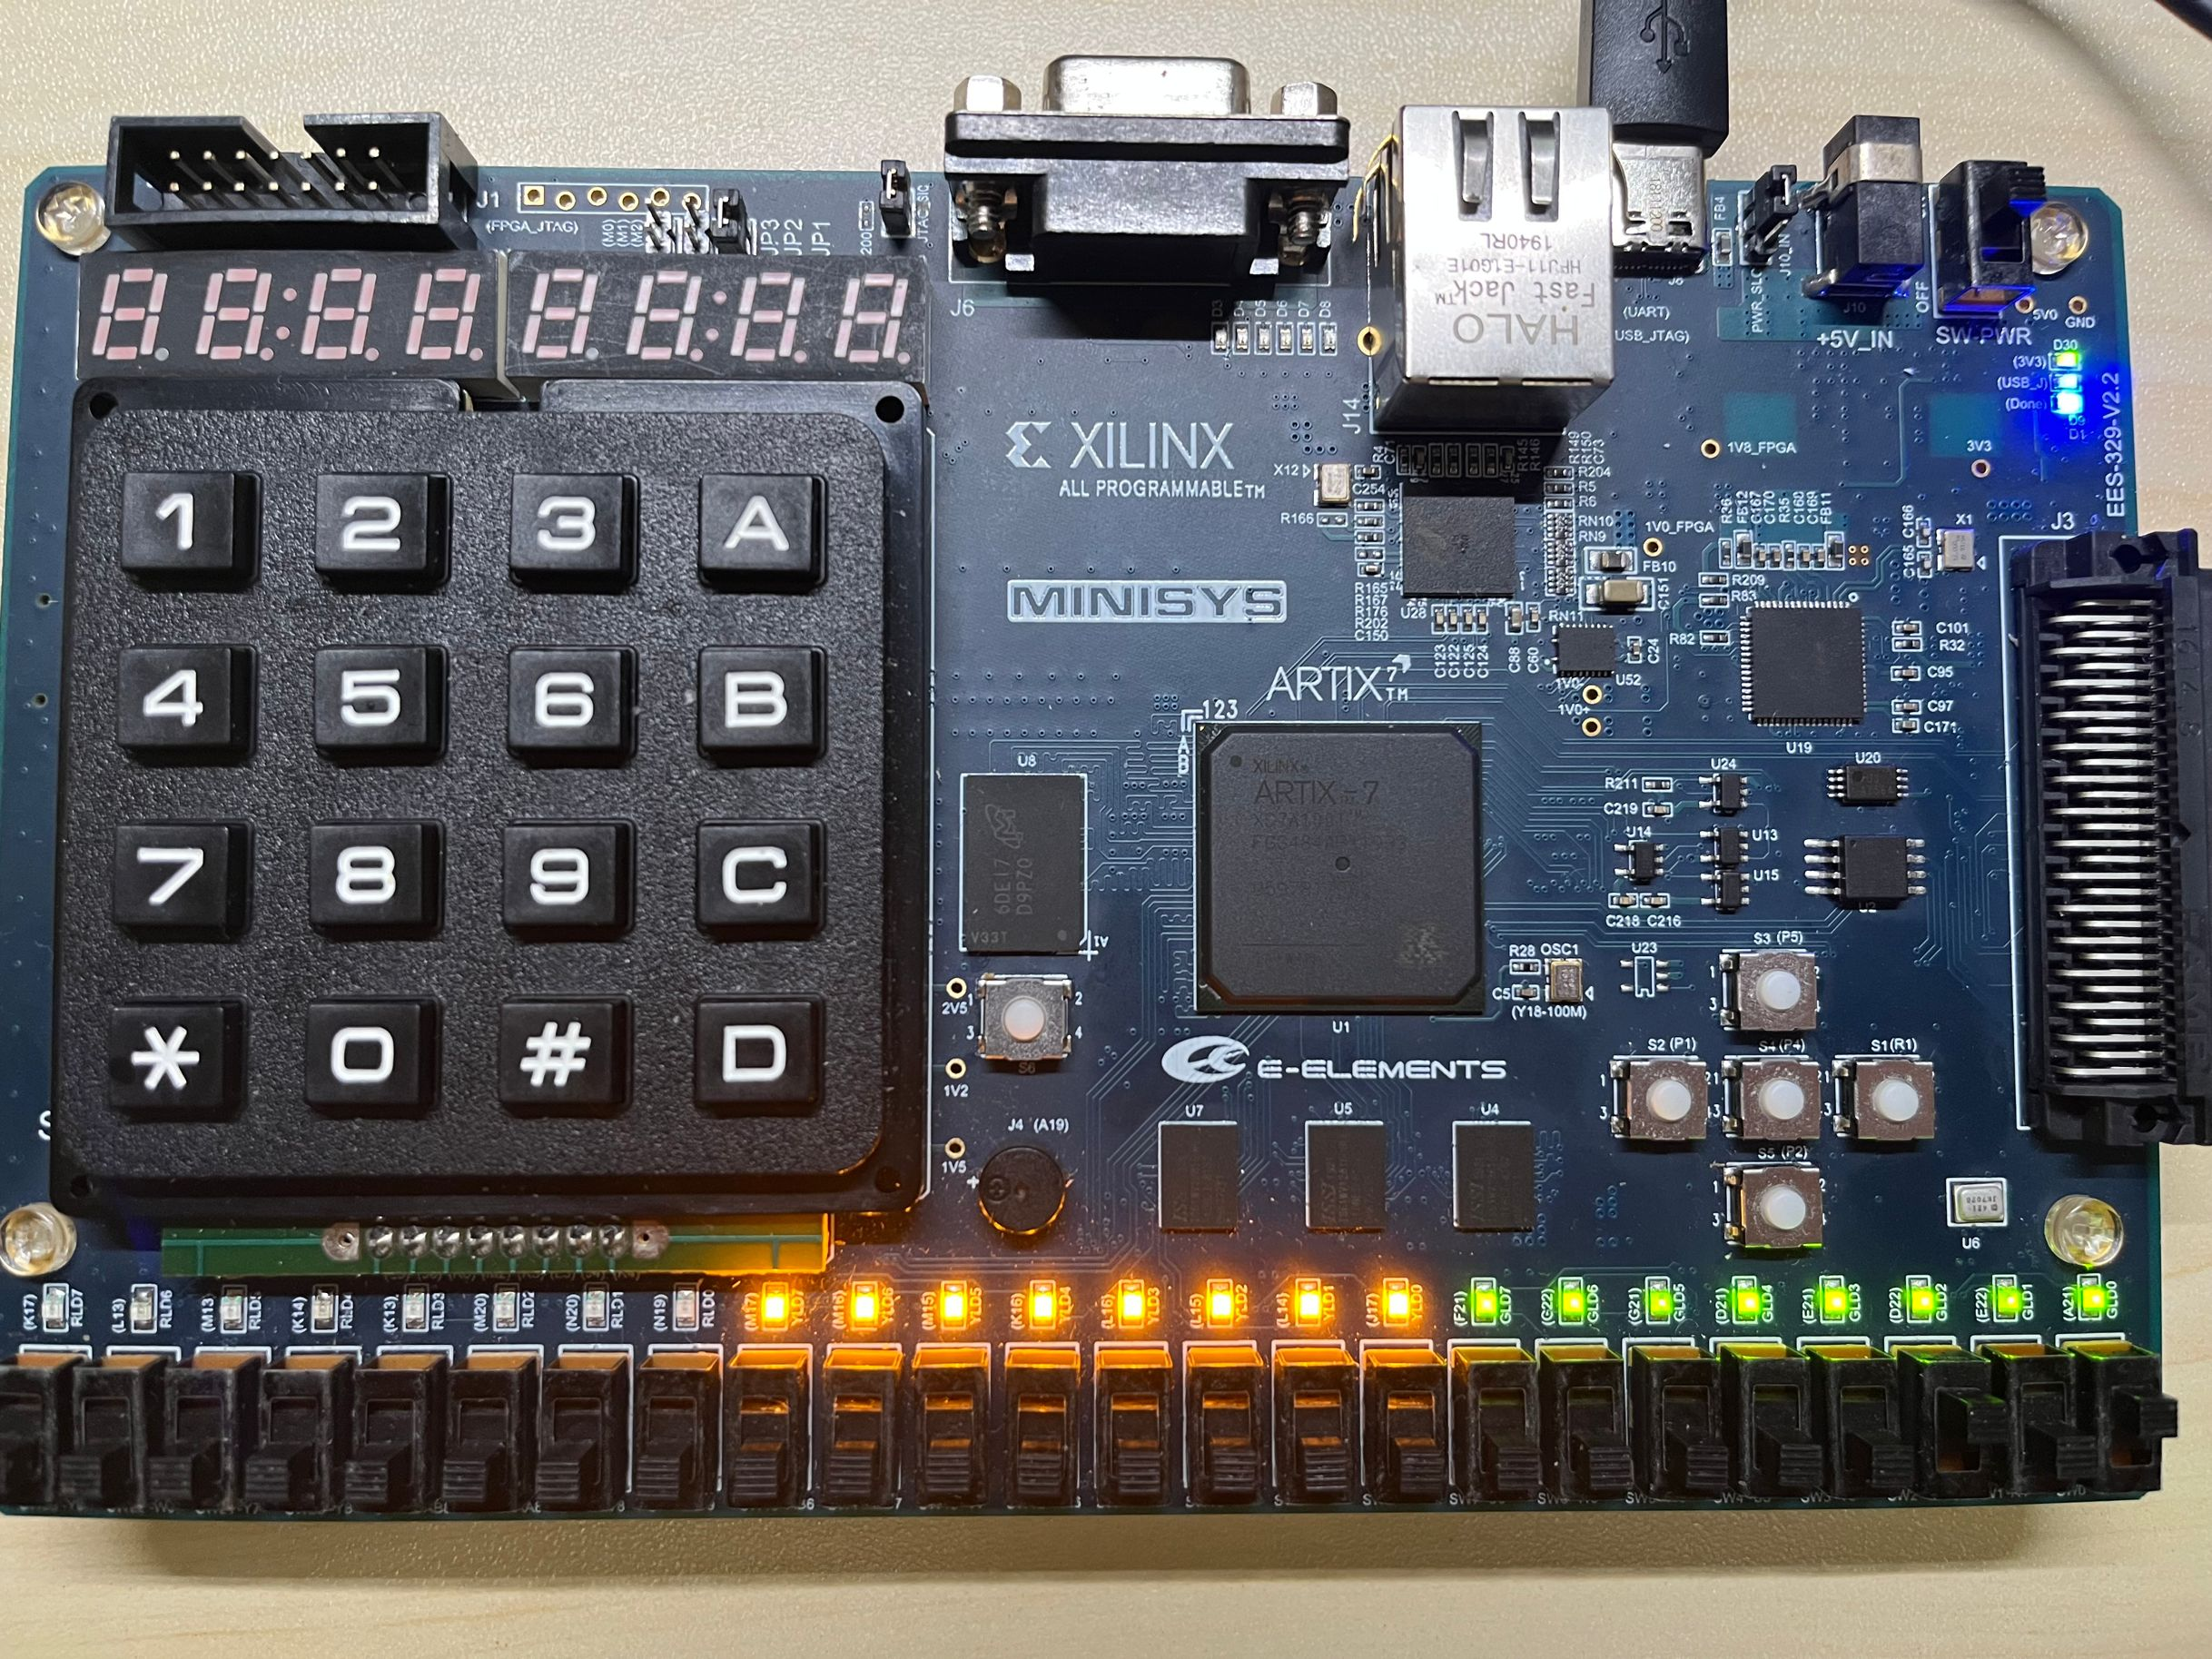
\includegraphics[width=0.5\textwidth]{fig/e1}
		\quad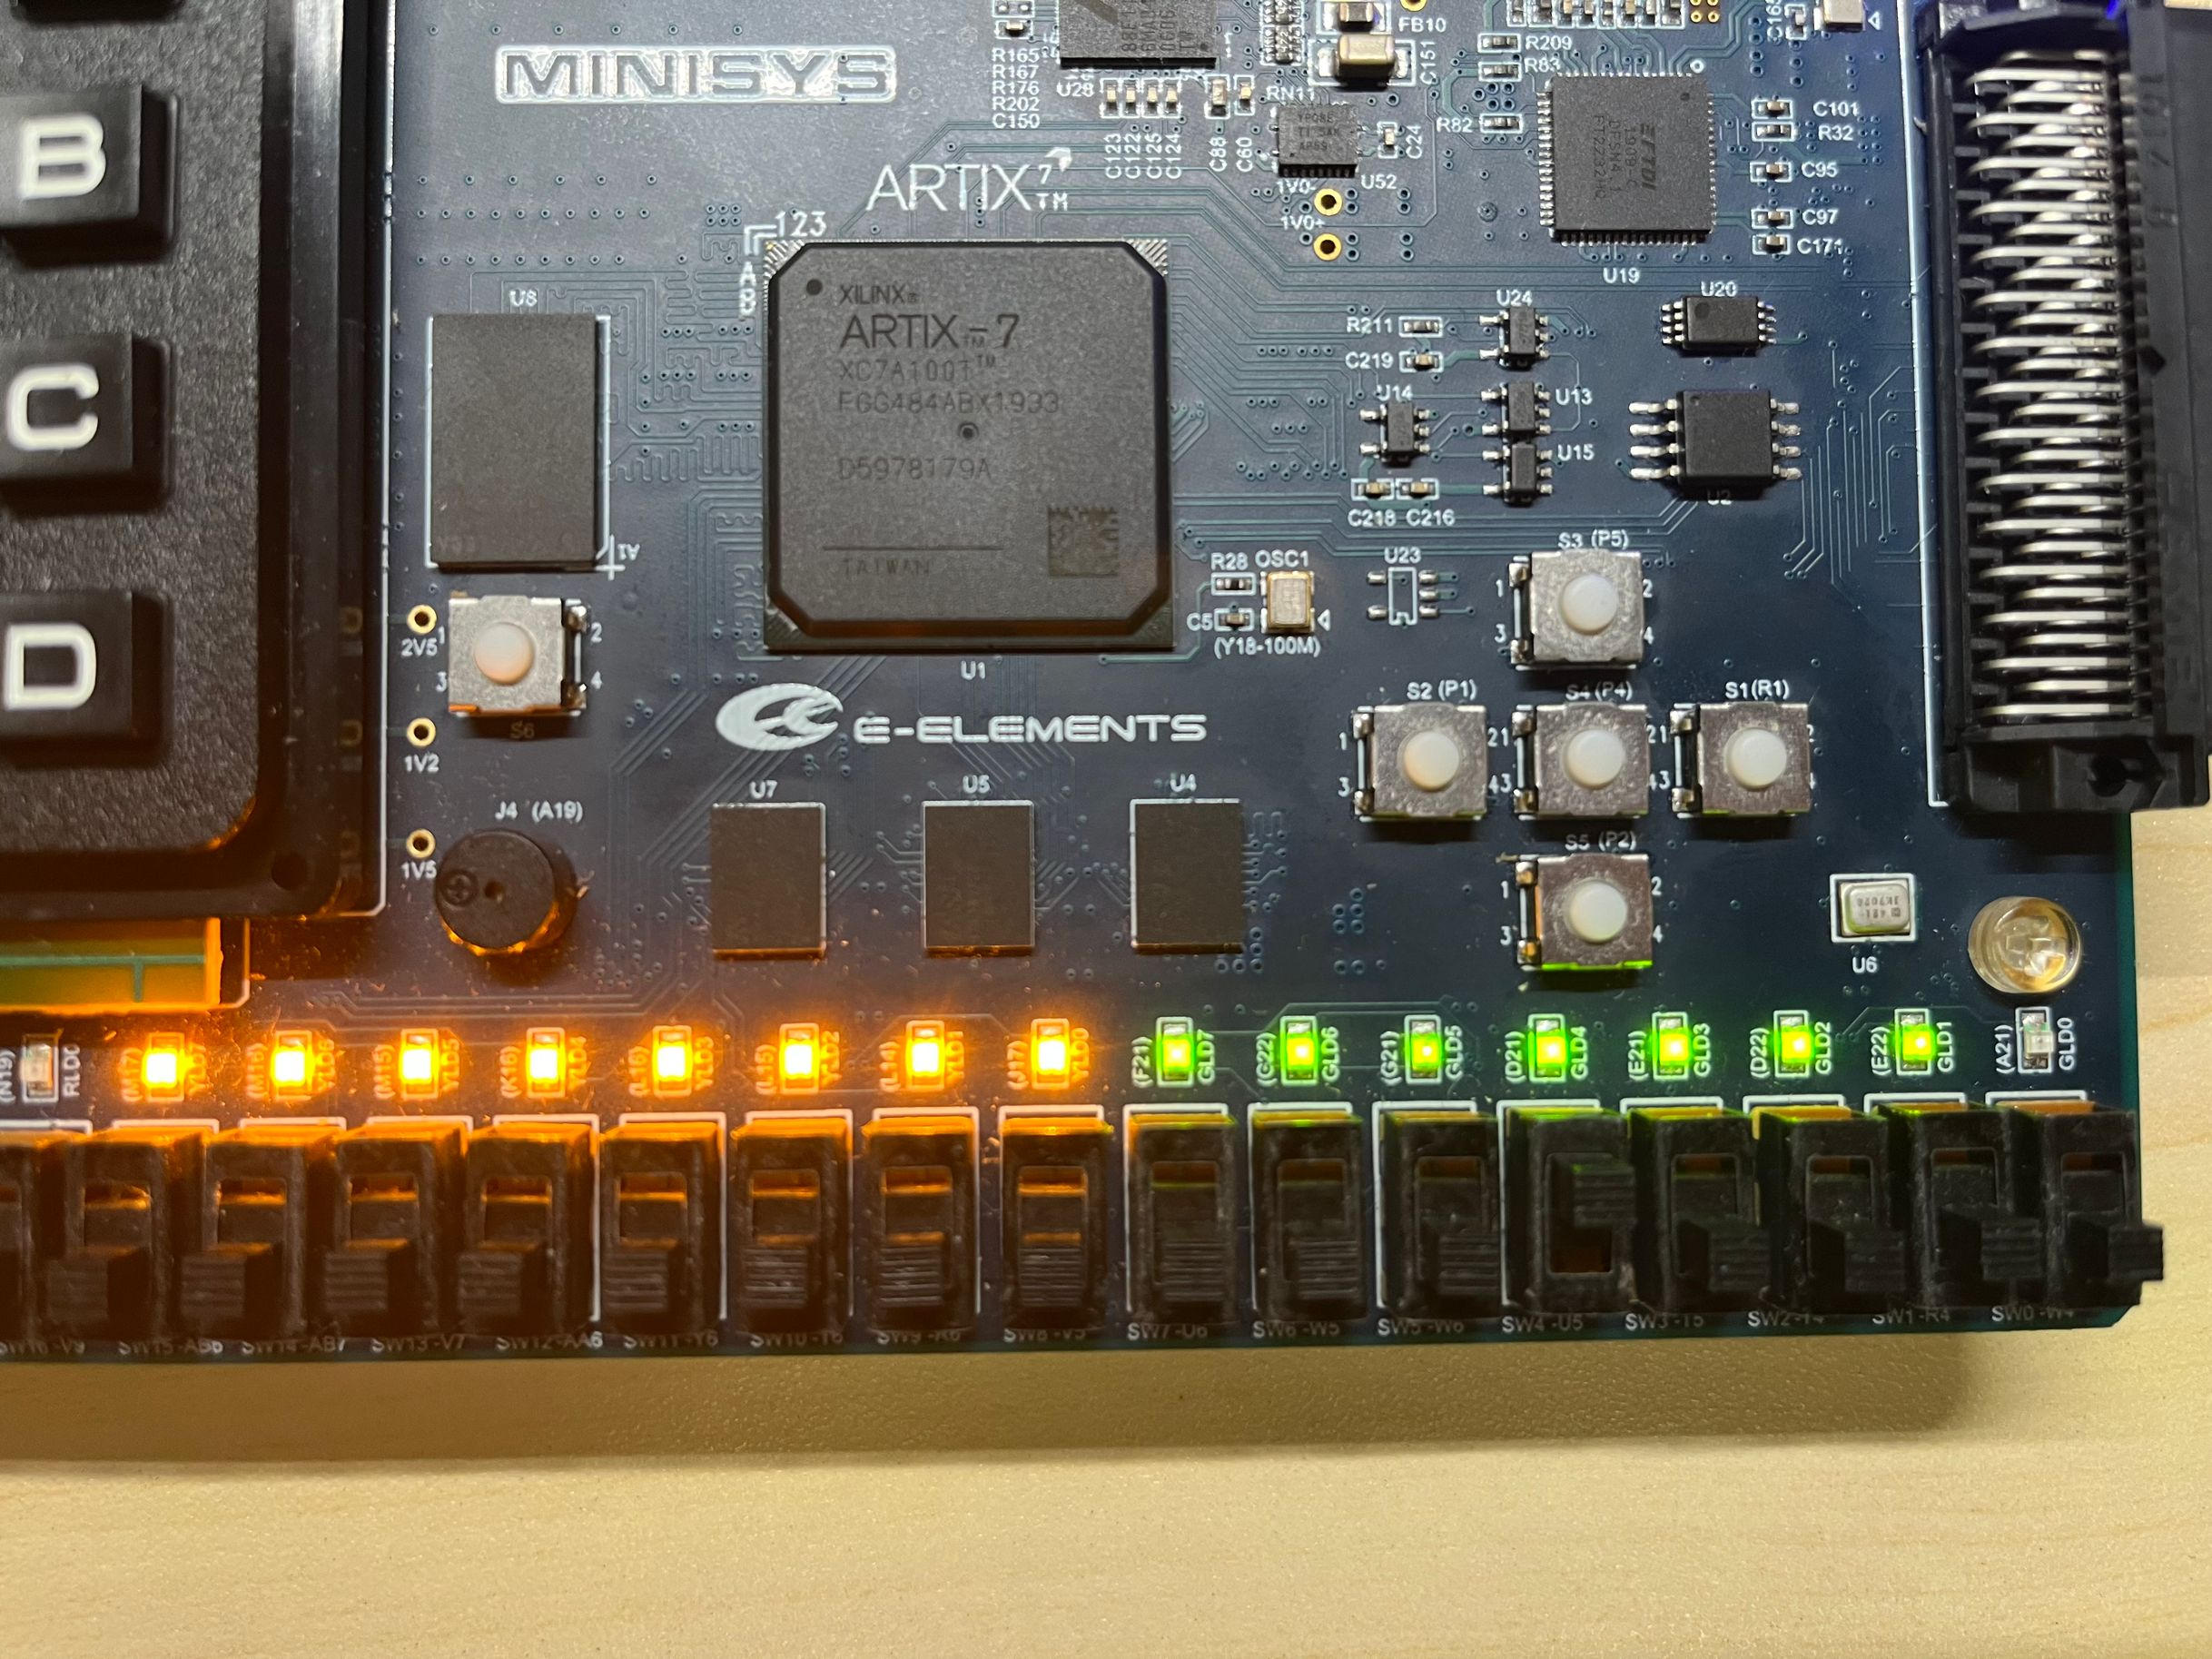
\includegraphics[width=0.5\textwidth]{fig/e2}}
\par The left fig. shows when decoder is not enabled (the 5$^{\text{th}}$ switch counting from right, a.k.a. dec\_en is set as 0 now), outputs are all 1. The right one, dec\_en = 1, A = B = C = D = 0, then Y[0] acts as the one-hot, since the output ports of 74138 is low-enabled, Y[0] = 0 and the rest 15 bits are 1.\\

\centerline{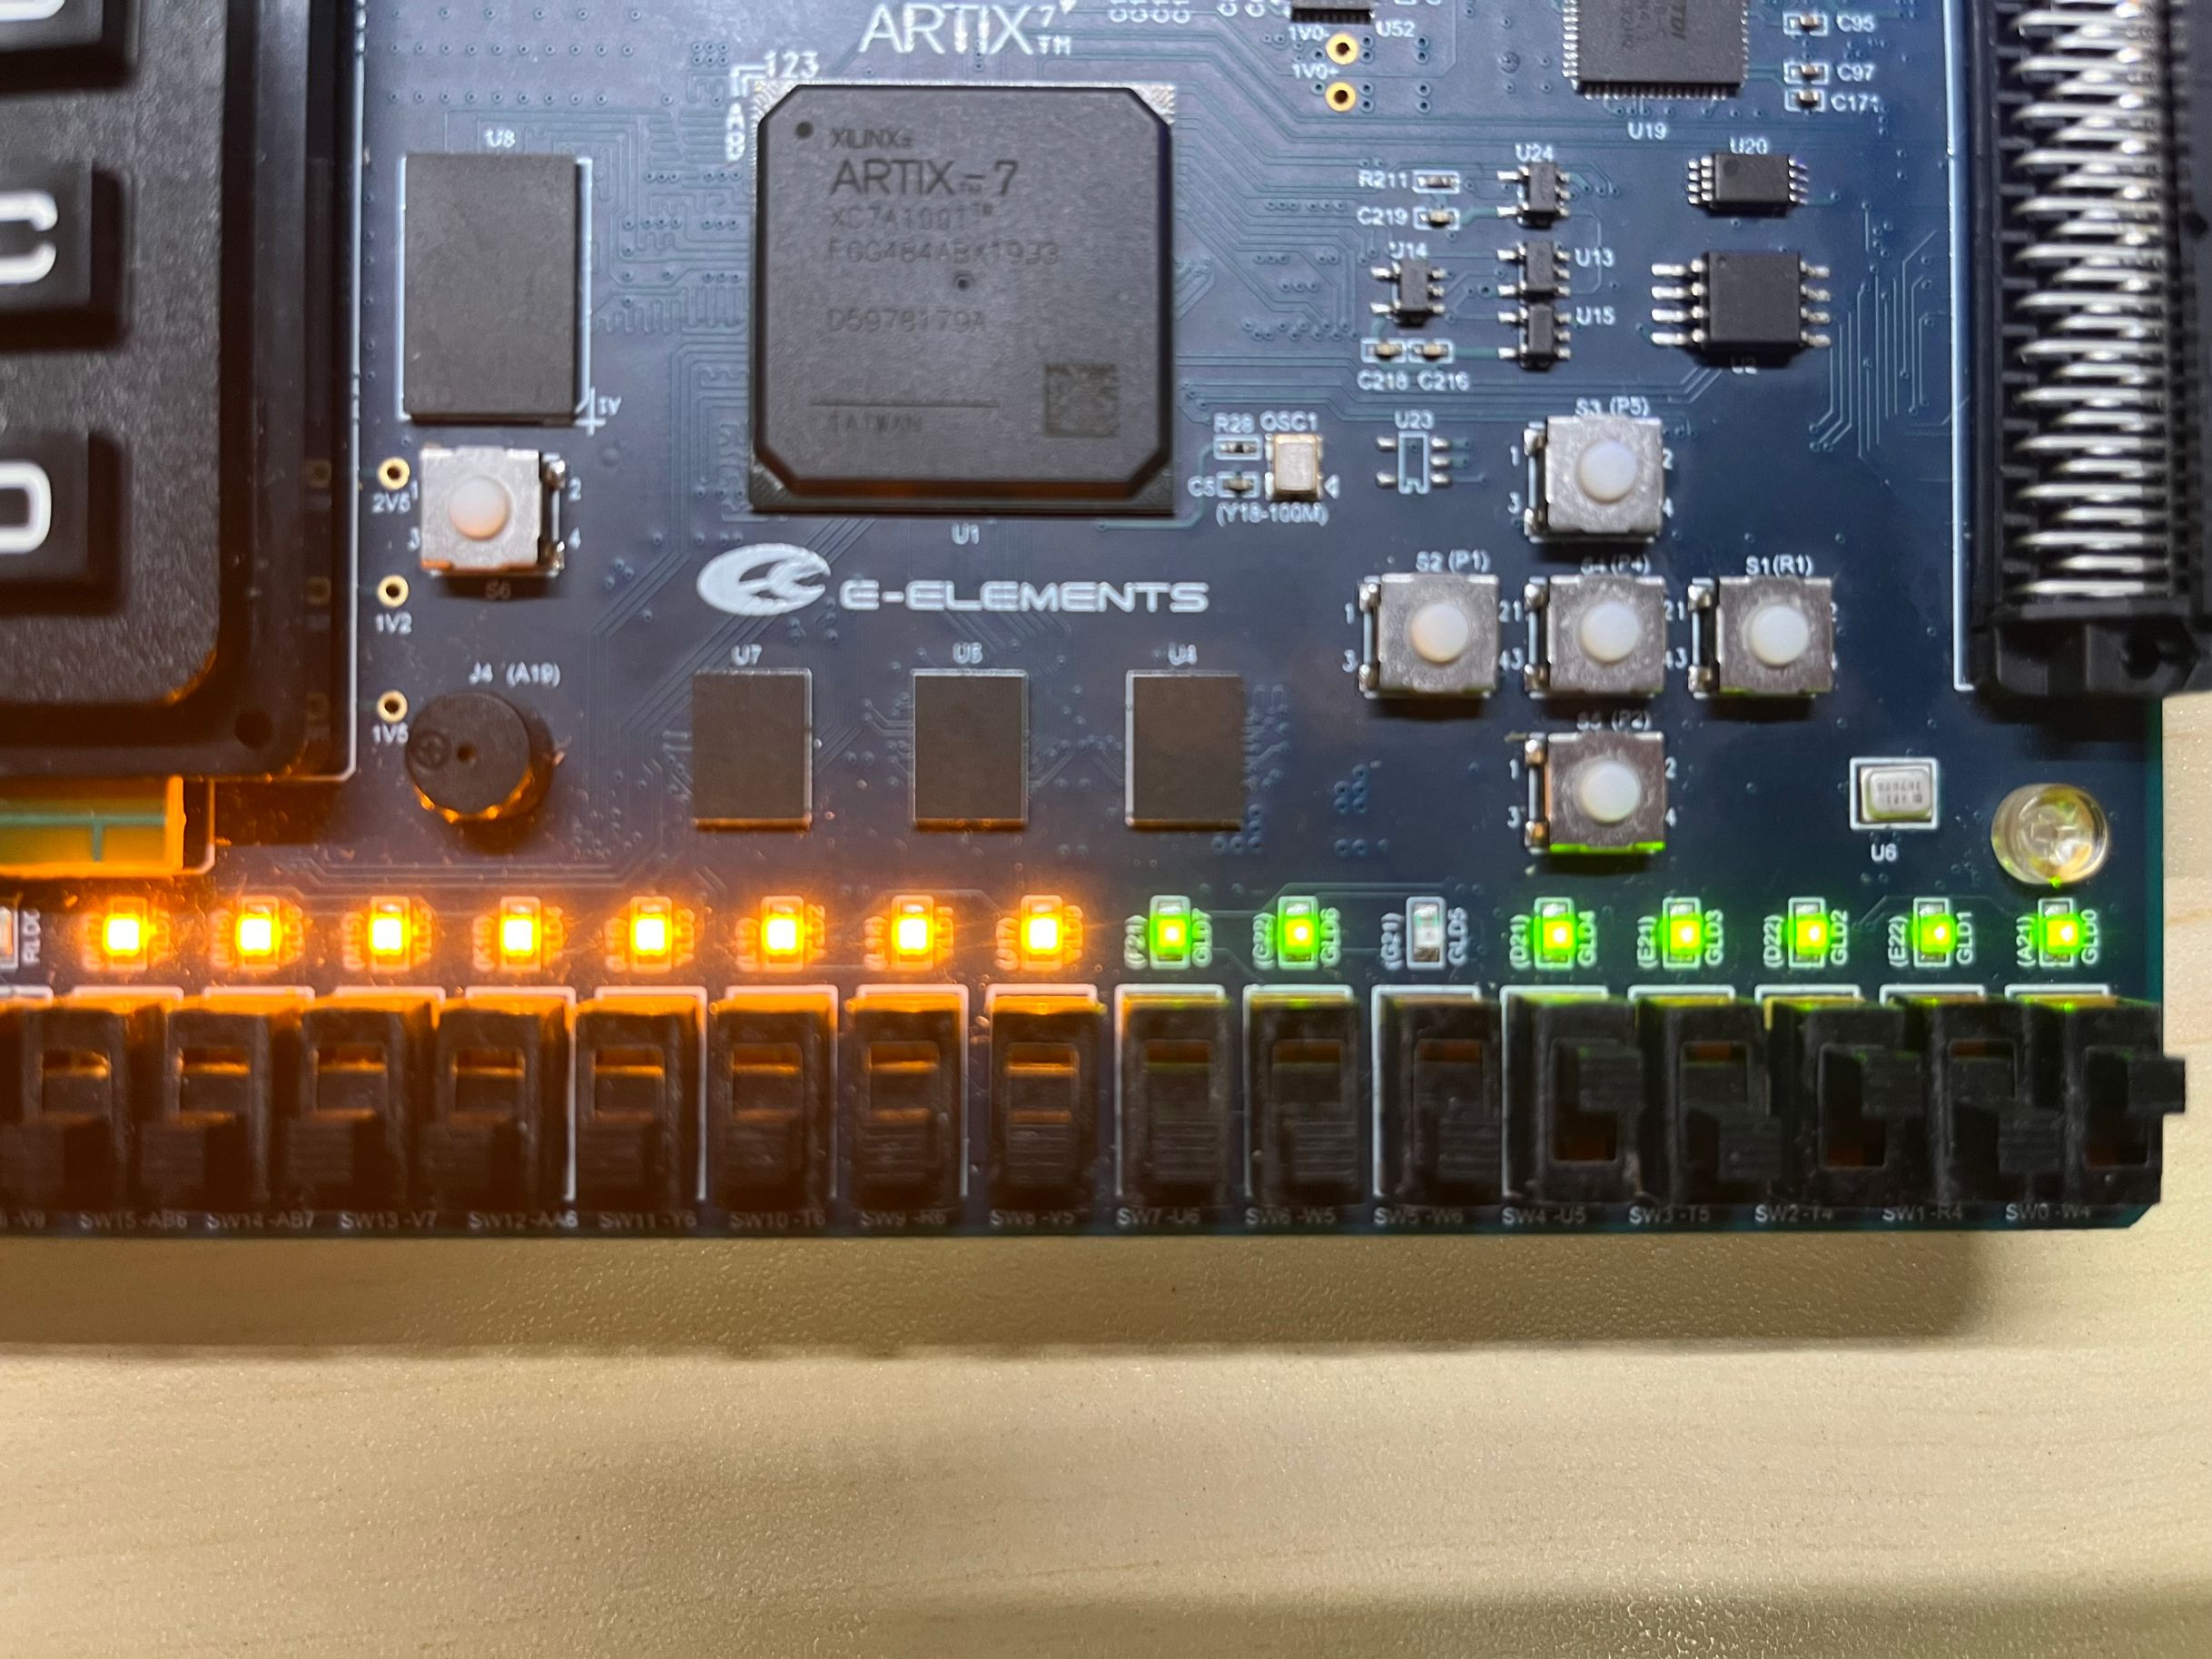
\includegraphics[width=0.33\textwidth]{fig/e3}
		\quad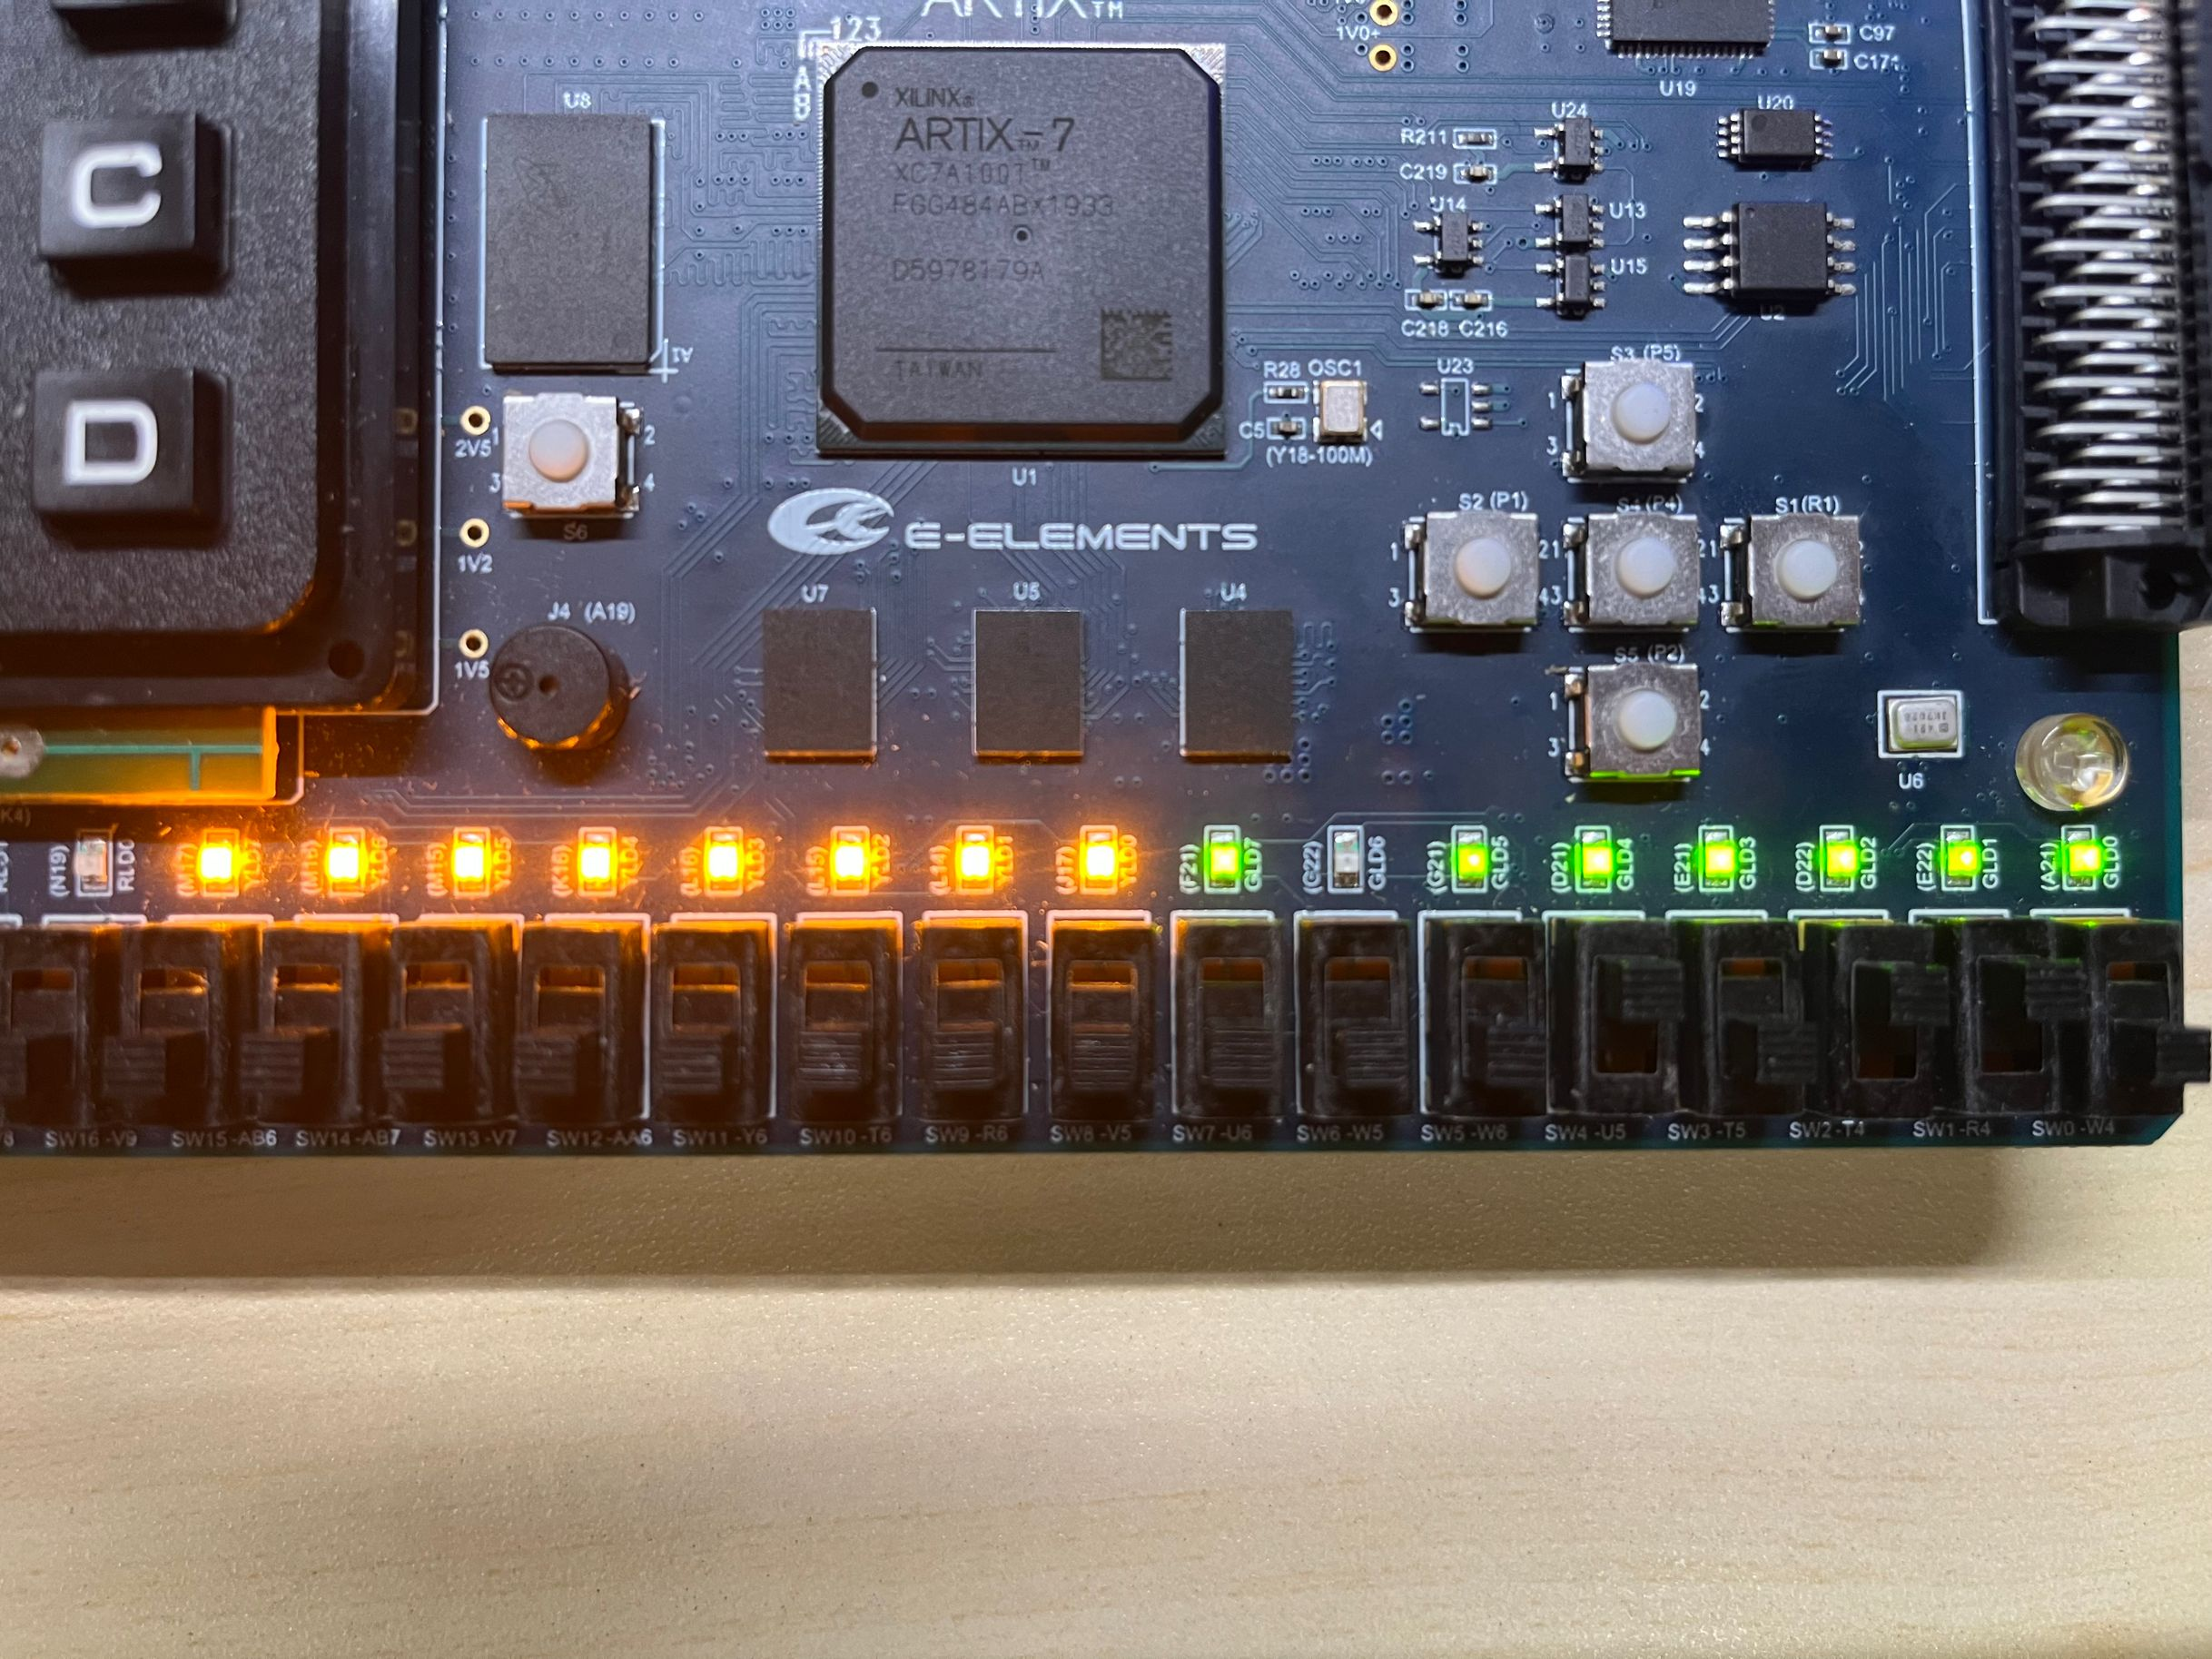
\includegraphics[width=0.33\textwidth]{fig/e4}
		\quad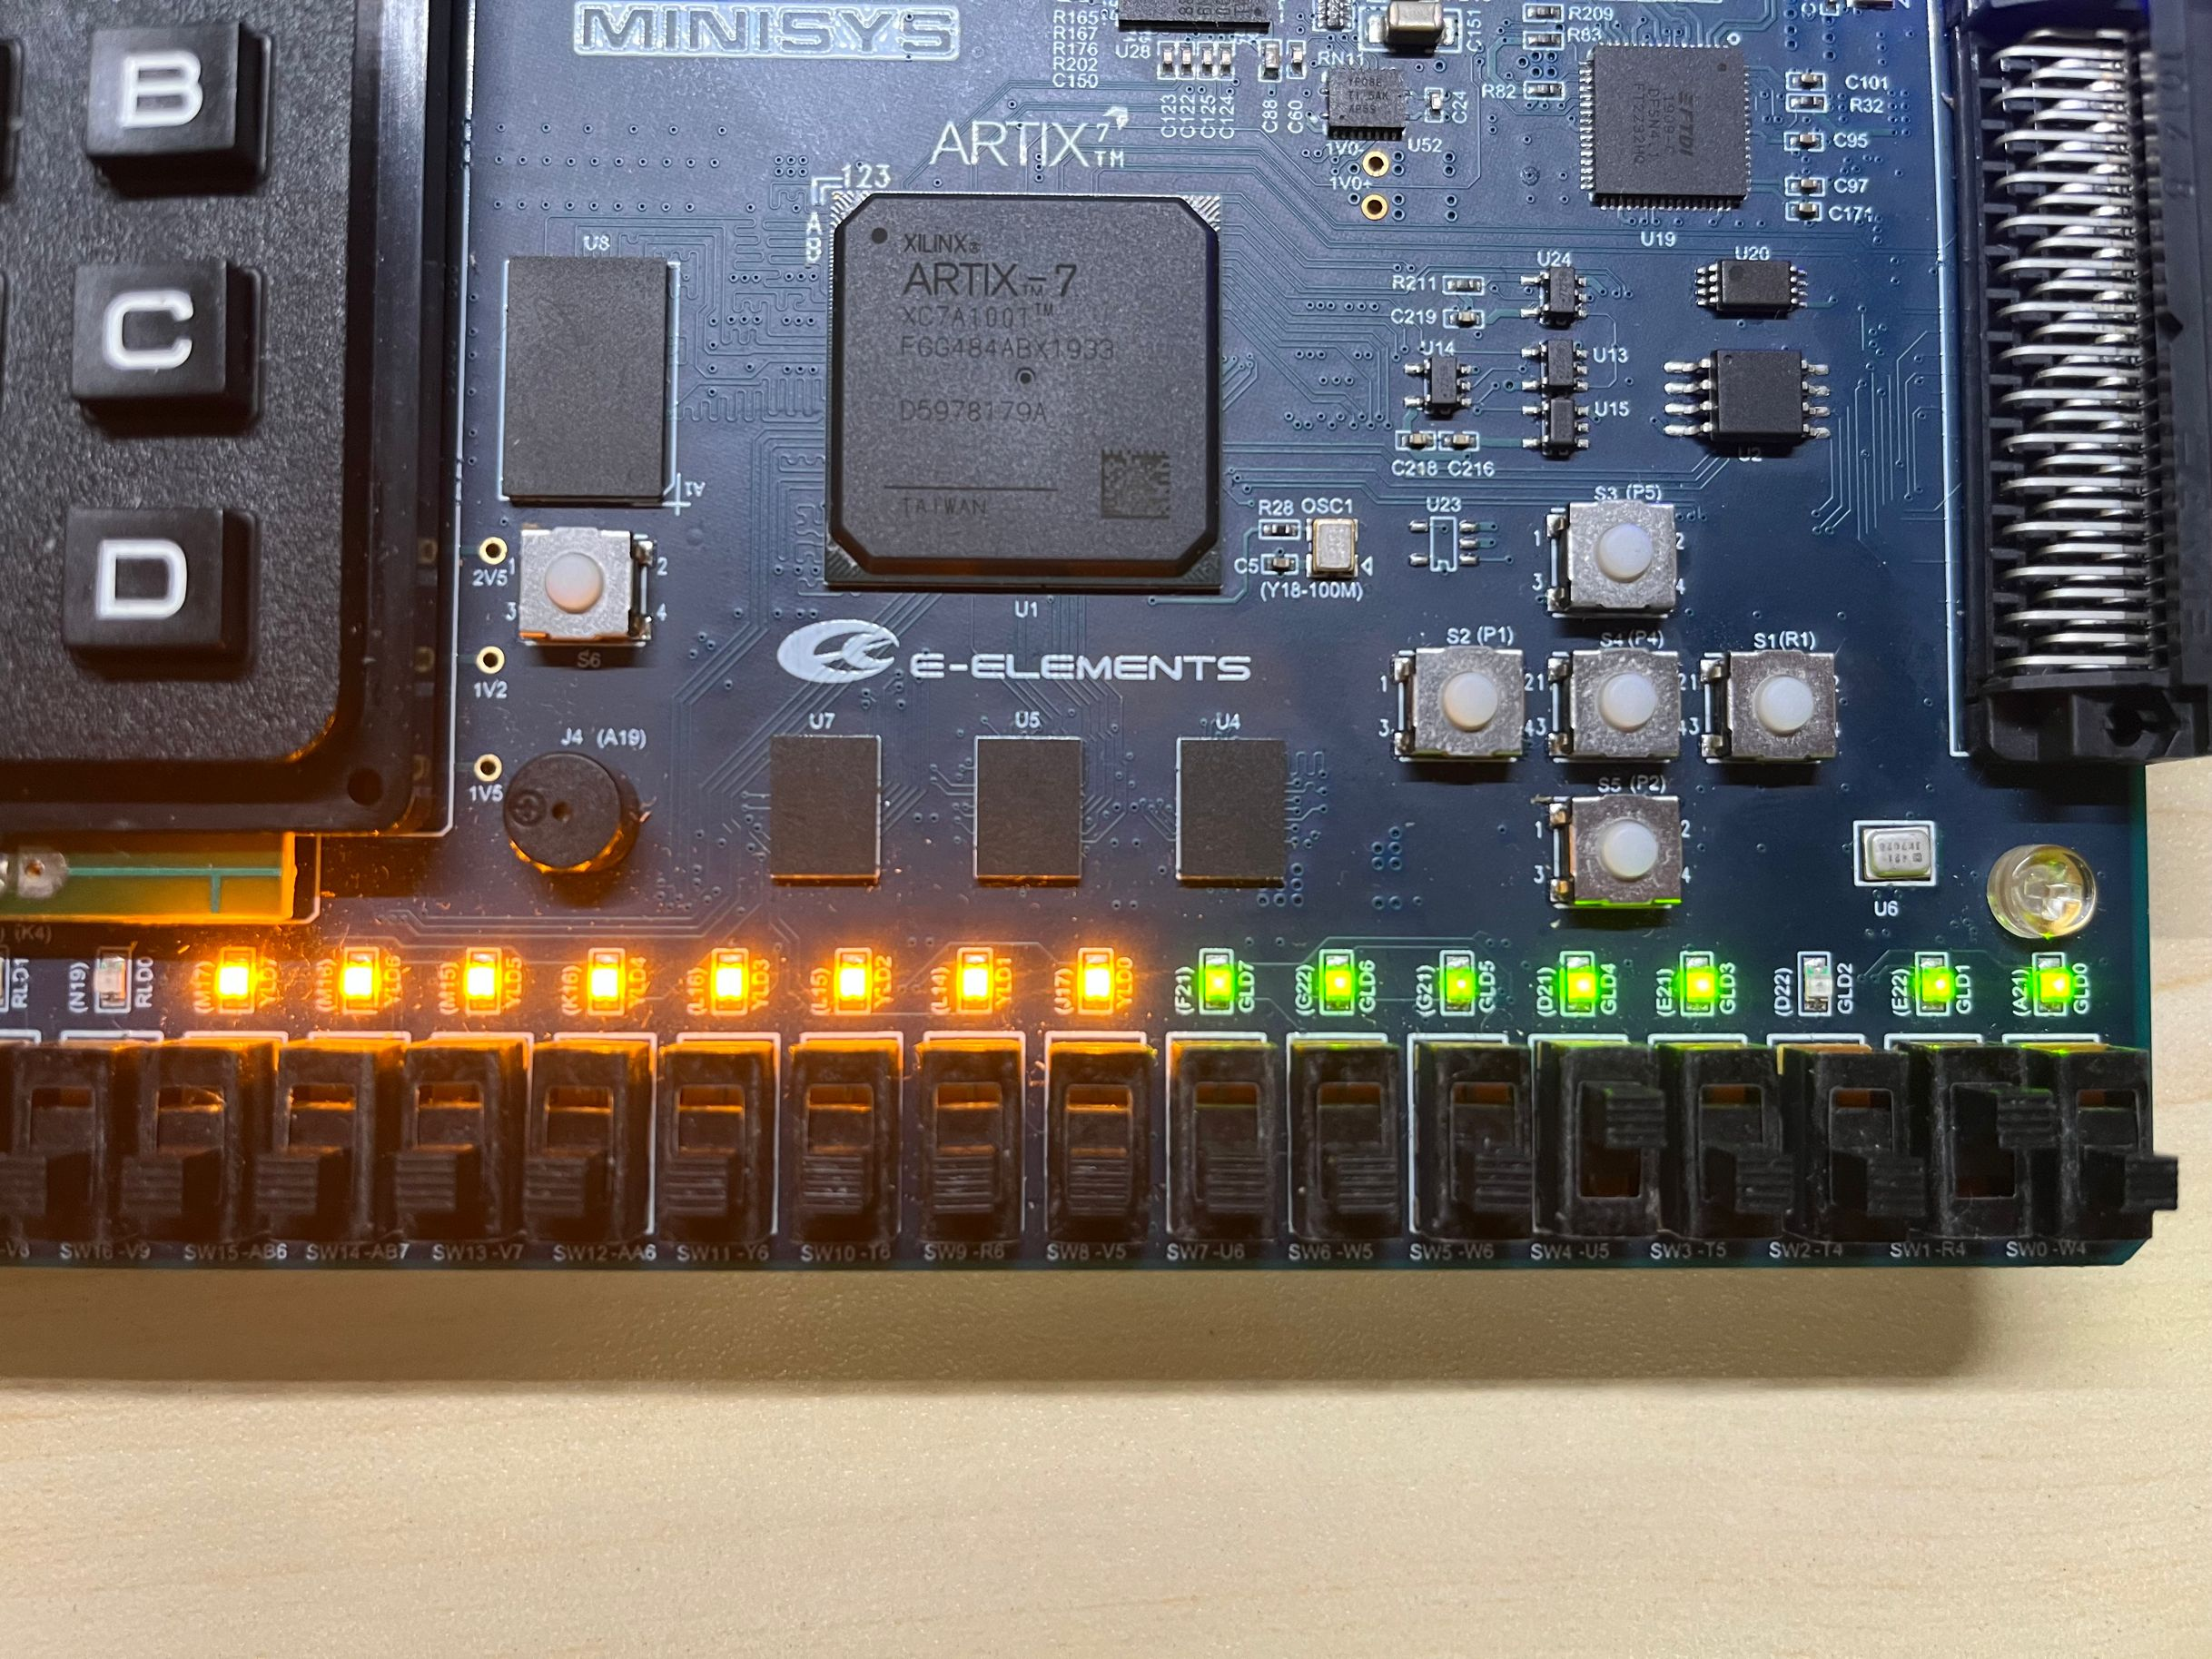
\includegraphics[width=0.33\textwidth]{fig/e5}}
\scriptsize
\noindent (a) input as 0101, output as Y[5] = 0, rest are 1; \qquad (b) input as 0110, output as Y[6] = 0, rest are 1;
\qquad (c) input as 0010, output as Y[2] = 0, rest are 1.
\normalsize


\subsection*{Task 2}
\subsubsection*{Design File}
\begin{lstlisting}
module mux_74151(
    input mux_en,
    input s2, s1, s0,
    input d0, d1, d2, d3, d4, d5, d6, d7,
    output reg Y,
    output W
);
    always @ * begin
        if (!mux_en) begin
            case ({s2, s1, s0})
                'd0: Y <= d0;
                'd1: Y <= d1;
                'd2: Y <= d2;
                'd3: Y <= d3;
                'd4: Y <= d4;
                'd5: Y <= d5;
                'd6: Y <= d6;
                'd7: Y <= d7;
            endcase
        end
        else begin
            Y <= 'b0;
        end
    end

    assign W = ~Y;
endmodule
\end{lstlisting}
\vspace{-3em}
\par As the same of standard 74151, the enable signal is low-enabled, and there should have two output ports, where one is the selected input and the other one is its negation.\\
\begin{lstlisting}
module func_df(
    input A, B, C, D,
    output Y
);
    assign Y = (~A & ~B & ~C & ~D) | (B & D) | (A & C) | (~B & C & ~D) | (~A & ~B & ~D);
endmodule
\end{lstlisting}

\begin{center}
\begin{karnaugh-map}[4][4][1][$AB$][$CD$]
\minterms{0,5,7,13,15,10,11,14,8}
\end{karnaugh-map}
\end{center}
\vspace{-2em}
From the K-map above (actually this is quite similar to checking the truth-table), we conclude:
\begin{lstlisting}
case ({A, B, C})
	'b000: Y = ~D;
	'b001: Y = ~D;
	'b010: Y = D;
	'b011: Y = D;
	'b110: Y = D;
	'b111: Y = 1;
	'b100: Y = 0;
	'b101: Y = 1;
endcase
\end{lstlisting}
\vspace{-3em}
Thus we map this into our module mux 74151:
\begin{lstlisting}
module func_1mux(
    input A, B, C, D,
    output Y
);
    mux_74151 mux(0, A, B, C,
                  ~D, ~D, D, D, 0, 1, D, 1,
                  Y);  // we don't use <W>, aka. ~Y
endmodule


module func_2mux(
    input A, B, C, D,
    output reg Y
);
    reg en1 = 1;
    reg en2 = 1;
    wire y1, y2;

    always @ * begin
        if (D) begin
            en1 <= 0;
            en2 <= 1;
            Y <= y1;
        end
        else begin
            en1 <= 1;
            en2 <= 0;
            Y <= y2;
        end
    end

    mux_74151 mux1(en1, A, B, C,
                   0, 0, 1, 1, 0, 1, 1, 1,
                   y1);  // D == 1

    mux_74151 mux2(en2, A, B, C,
                   1, 1, 0, 0, 0, 1, 0, 1,
                   y2);  // D == 0
endmodule
\end{lstlisting}

\subsubsection*{Simulation File}
\begin{lstlisting}
`timescale 1ns/1ps

module mux_74151_test();
    reg mux_en;
    reg s2, s1, s0;
    reg d0, d1, d2, d3, d4, d5, d6, d7;
    wire Y, W;

    mux_74151 mux(mux_en,
                  s2, s1, s0,
                  d0, d1, d2, d3, d4, d5, d6, d7,
                  Y, W);

    initial begin
        mux_en = 'b1;
        {s2, s1, s0} = 'b000;
        {d7, d6, d5, d4, d3, d2, d1, d0} = 'b1111_1111;

        #10 mux_en = 'b0;
        while ({s2, s1, s0} < 'b111) begin
            #10 {s2, s1, s0} = {s2, s1, s0} + 1;
            {d7, d6, d5, d4, d3, d2, d1, d0} = 'b0000_0001 << {s2, s1, s0};
        end
        #10 $finish();
    end
endmodule
\end{lstlisting}
\vspace{-2em}
\centerline{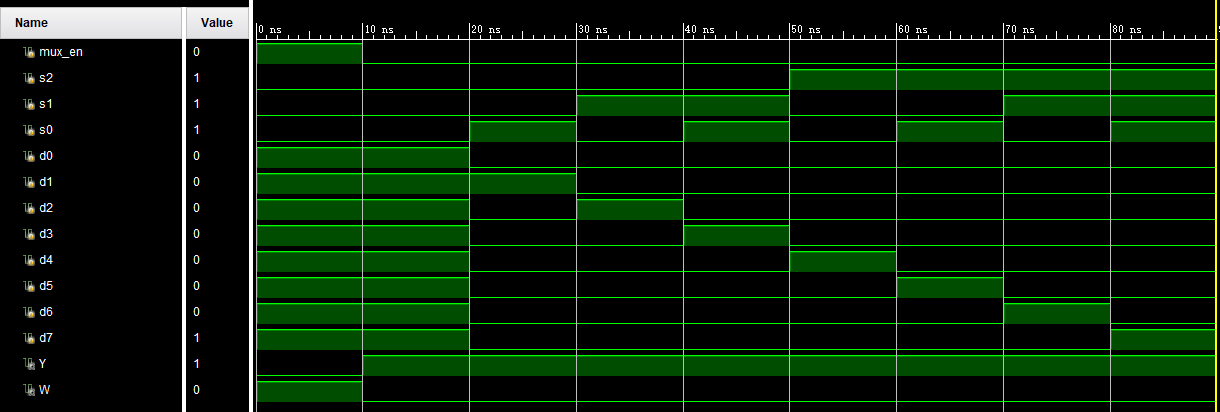
\includegraphics[width=\textwidth]{fig/t3}}
\par When testing the mux itself, we just take 1111\_1111 as an example input when it is not enabled (mux\_en == 1). When it is enabled, since the mux will output the cooresponding input d\$(x) where x = \{s2, s1, s0\}, and in the testbench we've let it to be one (while the others be zero), thus the output of mux, Y, should always be 1, and its negation, W, is always 0.

\begin{lstlisting}
`timescale 1ns/1ps

module mux_func_test();
    reg A, B, C, D,
    wire Y_df, Y_1mux, Y_2mux;

    func_df df(A, B, C, D, Y_df);
    func_1mux one_mux(A, B, C, D, Y_1mux);
    func_2mux two_mux(A, B, C, D, Y_2mux);

    initial begin
        {A, B, C, D} = 'b0000;
        while ({A, B, C, D} < 'b1111) begin
            #10 {A, B, C, D} = {A, B, C, D} + 1;
        end
        #10 $finish();
    end
endmodule
\end{lstlisting}
\vspace{-2em}
\centerline{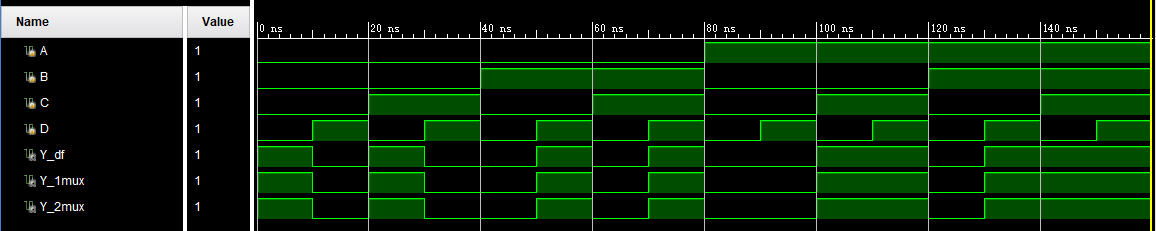
\includegraphics[width=\textwidth]{fig/func}}
\par First we notice that three ways to implement the function have the same output, then we check the truth-table and found all the outputs are right.
\begin{longtable}{cccc|c}
\hline
A & B & C & D & Y \\ \hline
\endfirsthead
%
\endhead
%
\hline
\endfoot
%
\endlastfoot
%
0 & 0 & 0 & 0 & 1 \\
0 & 0 & 0 & 1 & 0 \\
0 & 0 & 1 & 0 & 1 \\
0 & 0 & 1 & 1 & 0 \\
0 & 1 & 0 & 0 & 0 \\
0 & 1 & 0 & 1 & 1 \\
0 & 1 & 1 & 0 & 0 \\
0 & 1 & 1 & 1 & 1 \\
1 & 0 & 0 & 0 & 0 \\
1 & 0 & 0 & 1 & 0 \\
1 & 0 & 1 & 0 & 1 \\
1 & 0 & 1 & 1 & 1 \\
1 & 1 & 0 & 0 & 0 \\
1 & 1 & 0 & 1 & 1 \\
1 & 1 & 1 & 0 & 1 \\
1 & 1 & 1 & 1 & 1 \\ \hline
\end{longtable}


\subsection*{Problems \& Solutions}
\paragraph{(1)}At first I couldn't understand why 74138-decoder should has three enable ports, until detailed research \textit{"The three enable pins of chip (in which Two active-low and one active-high) reduce the need for external gates or inverters when expanding."} (Components101, 2018)
\paragraph{(2)}After happening the dilemma that variables went to be X again in the simulation, I have a better understanding of blocking and non-blocking assignments.

\end{document}